We now turn to universality for random matrices: eigenvalue statistics of symmetric random matrices are largely independent of the distribution of the entries. This can be viewed as an analogue of the CLT, but now instead of a simple sum the manipulation of the random variables involves computation of eigenvalues.  In particular, we will look at both \emph{global statistics}, i.e., what do histograms of all eigenvalues look like, and \emph{local statistics}, i.e., what do histograms of the largest eigenvalue look like. For the theory we focus on the global statistics (as proving results for the local statistics requires much more sophisticated  mathematical tools and the formula for the distribution involves \href{https://en.wikipedia.org/wiki/Painlevé_transcendents}{Painlevé transcendents} with no exact formula), and in particular, we focus on the phenomenon that symmetric matrices with independent, identically distributed (iid) entries have global statistics that look like the \emph{semicircle}:
\[
{\sqrt{4-x^2} \over 2\ensuremath{\pi}} \qquad \text{for } x \in [-2, 2].
\]
The \emph{semicircle distribution} can in multiple ways be viewed as a random matrix analogue of  the \emph{normal distribution} $\ensuremath{\scrN}$.

In this section we will show universality again using the \emph{Method of Moments}: we will show that the moments of the eigenvalue statistics converge to the moments of a known distribution. For a scalar random variable $X$ the distribution is generally encoded by the standard moments:
\[
\ensuremath{\bbE} X^k
\]
We will see that in the matrix case the global distribution of eigenvalues is encoded by the matrix-analogue of moments: for $A_n \ensuremath{\in} \ensuremath{\bbR}^{n \ensuremath{\times} n}$ we define
\[
\ensuremath{\bm{\mathrm{E}}} A_n^k := {1 \over n} \ensuremath{\bbE} \Tr A_n^k
\]
where $\Tr$ is the trace of a matrix (sum of the diagonal).  It may not be obvious but these simple matrix-versions of "expectations" are equivalent to moments of the eigenvalue distribution. As the dimension of the matrix becomes large ($n \ensuremath{\rightarrow} \ensuremath{\infty}$) we will show these matrix moments tend to the moments of a semicircle.

Note that moments are only guaranteed to uniquely define a density in the special case where the probability density decays sufficiently fast, but this is something the Gaussian and semicircle both satisfy.

\textbf{Further reading}: \href{https://terrytao.wordpress.com/wp-content/uploads/2011/02/matrix-book.pdf}{Topics in Random Matrix Theory} by Terry Tao gives a more advanced, higher level introduction to random matrix theory, though perhaps too high a level for most 1st year students. The field of Random Matrix Theory and universality grew out of a beautiful collaboration between theoretical physcists, statisticians, and pure mathematics and involves the synthesis of tools between these different areas.

\section{Experimental observation of universality}
As a simple example,  consider $A_n \ensuremath{\in} \ensuremath{\bbR}^{n \ensuremath{\times} n}$ which is symmetric ($A_n = A_n^\ensuremath{\top}$) and whose entries on and above the diagonal are iid random variables taking values $\ensuremath{\pm}1$ with equal probability (and entries below the diagonal defined by symmetry). Each sample of $A_n$ will have $n$ eigenvalues, which we denote $\ensuremath{\sigma}(A_n) = \set{\ensuremath{\lambda}_1,\ensuremath{\ldots},\ensuremath{\lambda}_n}$ (for concreteness we can assume they are sorted from smallest to largest). If we plot a histogram of rescaled eigenvalues $\ensuremath{\sigma}(A_n/ \sqrt{n}) = \set{{\ensuremath{\lambda}_1 \over \sqrt{n}}, \ensuremath{\ldots}, {\ensuremath{\lambda}_n \over \sqrt{n}}}$ of a \emph{single sample} $A_n$ we get a semicircle:


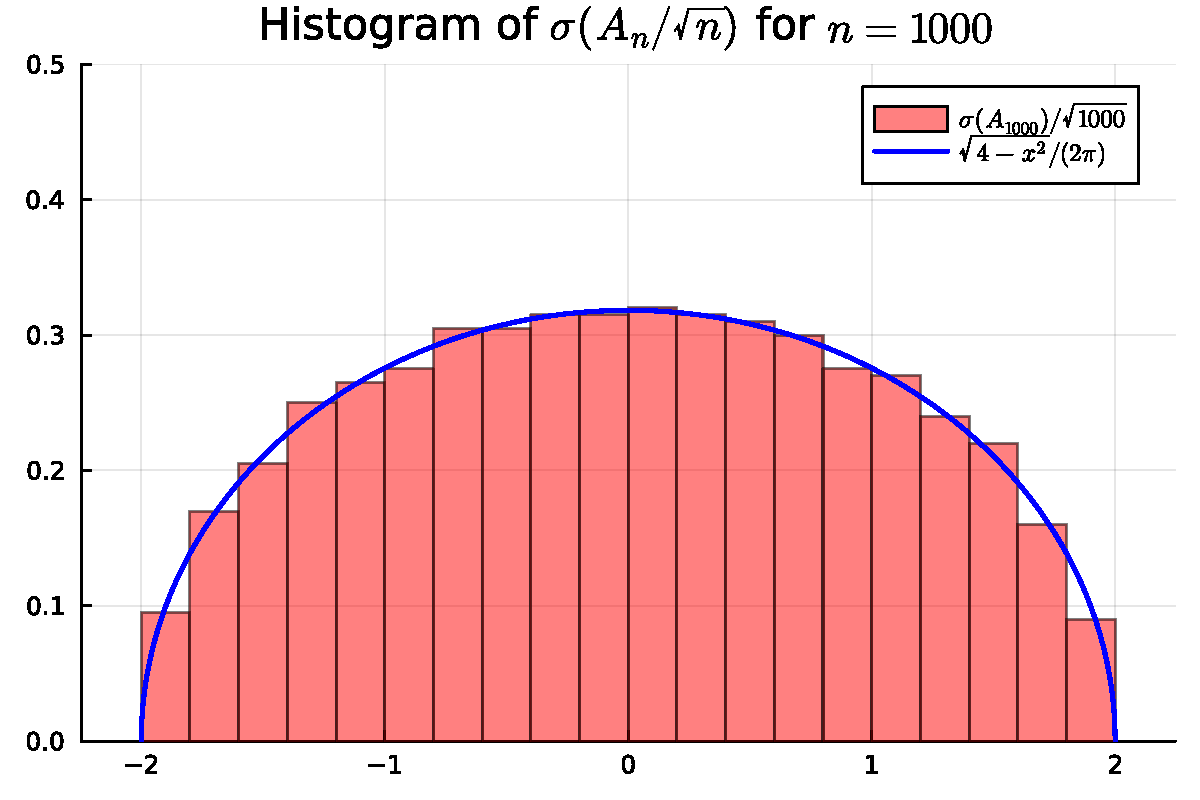
\includegraphics[width=0.6\linewidth,height=0.45\linewidth]{figures/II.Universality_1_1.pdf}

Just as in the CLT, this phenomena is independent of the distribution of the entries of $A_n$ provided the moments are finite: we always get a semicircle (shifted and scaled to match the mean and variance).

Like the CLT we will show this observation using the Method of Moments, and again we can deduce the moments experimentally by letting $n$ increase (a single sample per $n$ works in this case):


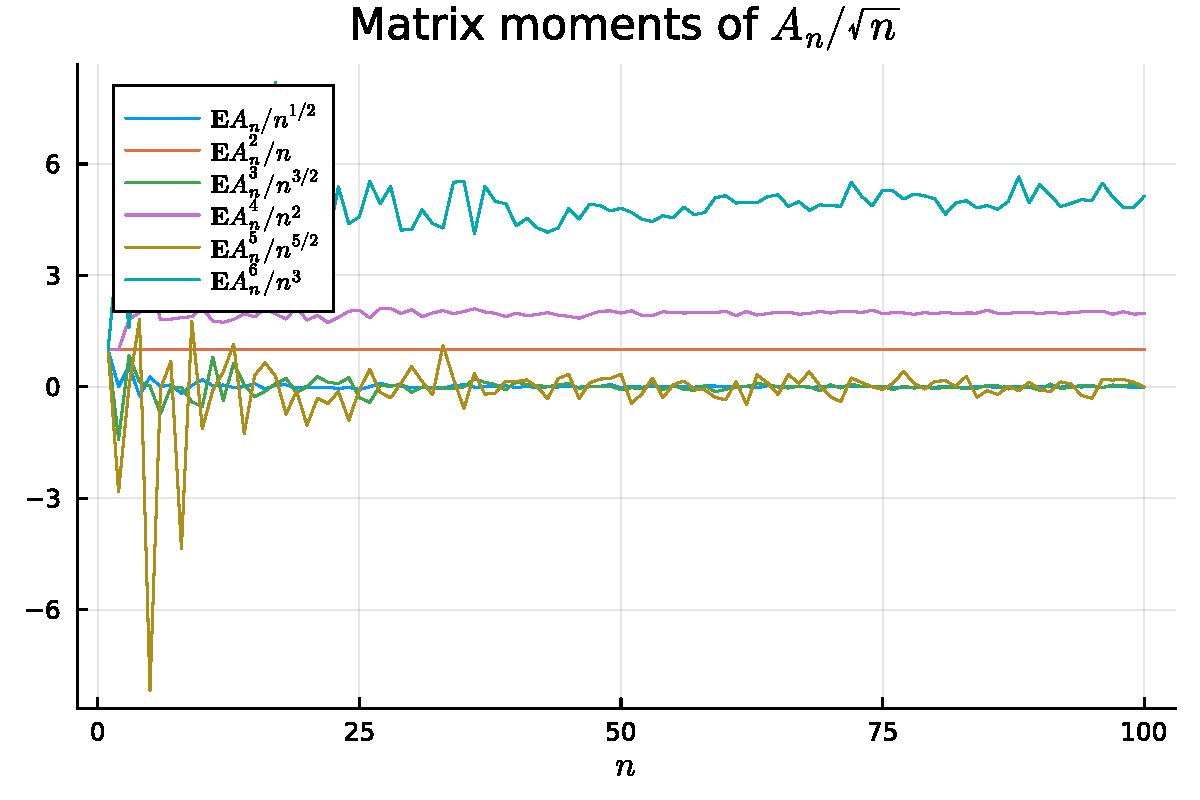
\includegraphics[width=0.6\linewidth,height=0.45\linewidth]{figures/II.Universality_2_1.pdf}

Again the odd moments appear to be zero but now we might conjecture that the even moments satisfy
\[
\ensuremath{\bm{\mathrm{E}}}A_n^2/n \ensuremath{\rightarrow} 1,\quad \ensuremath{\bm{\mathrm{E}}}A_n^4/n^2 \ensuremath{\rightarrow} 2,\quad \ensuremath{\bm{\mathrm{E}}}A_n^6/n^3 \ensuremath{\rightarrow} 5.
\]
Again we are left with the tasks of: (1) deducing an exact formula for these moments, and (2) proving that the semicircle has the same moments.

\section{Wigner ensembles and global statistics}
To discuss universality in the setting of random matrices we focus on symmetric matrices with iid entries, i.e., the \emph{Wigner ensembles}:

\begin{definition}[Wigner] A random matrix $A_n \ensuremath{\in} \ensuremath{\bbR}^{n \ensuremath{\times} n}$ is a Wigner matrix if:

\begin{itemize}
\item[1. ] The entries $a_{kj}$ for $j \ensuremath{\geq} k$ are all iid with mean 0, variance 1, and all moments are finite.


\item[2. ] The matrix $A_n$ is symmetric: $a_{kj} = a_{jk}$.

\end{itemize}
\end{definition}

We are interested in the global distribution of the eigenvalues. A Wigner ensemble $A_n \ensuremath{\in} \ensuremath{\bbR}^{n \ensuremath{\times} n}$ has $n$ eigenvalues $\ensuremath{\lambda}_1, \ensuremath{\ldots}, \ensuremath{\lambda}_n$ which can be viewed as $n$ random variables in their own right. The probability density associated with their histogram is described in terms of the moments:
\[
\ensuremath{\sigma}_{nk} := {1 \over n} \ensuremath{\bbE}[\ensuremath{\lambda}_1^k + \ensuremath{\ldots} + \ensuremath{\lambda}_n^k].
\]
It's a little delicate explaining why these encode the distribution of the histogram so we will just take it for granted in what follows.

We want to show that as $n \ensuremath{\rightarrow} \ensuremath{\infty}$ that these go to the moments of the semicircle. But before that we observe that we can rewrite these moments in terms of $A_n$ itself. Recall the following:

\begin{proposition}[Cyclic property of trace] For any $A \ensuremath{\in} \ensuremath{\bbR}^{n \ensuremath{\times} m}$ and $B \ensuremath{\in} \ensuremath{\bbR}^{m \ensuremath{\times} n}$ we have
\[
\Tr[A B] = \Tr[B A]
\]
for the trace $\Tr A_n = a_{11} + \ensuremath{\cdots} + a_{nn}$.

\end{proposition}
\textbf{Proof} We show this by direct inspection:
\meeq{
\Tr A B = \ensuremath{\sum}_{k=1}^n \ensuremath{\bm{\e}}_k^\ensuremath{\top} A B \ensuremath{\bm{\e}}_k = \ensuremath{\sum}_{k=1}^n  \begin{bmatrix} a_{k1} & \ensuremath{\cdots} & a_{km} \end{bmatrix} \begin{bmatrix} b_{1k} \\ \ensuremath{\vdots} \\ b_{m1} \end{bmatrix} = \ensuremath{\sum}_{k=1}^n \ensuremath{\sum}_{j=1}^m a_{kj} b_{jk} \ccr
  = \ensuremath{\sum}_{j=1}^m \ensuremath{\sum}_{k=1}^n b_{jk} a_{kj} = \ensuremath{\sum}_{j=1}^m \begin{bmatrix} b_{j1} & \ensuremath{\cdots} & b_{jn} \end{bmatrix} \begin{bmatrix} a_{j1} \\ \ensuremath{\vdots} \\ a_{jn} \end{bmatrix} = \ensuremath{\sum}_{j=1}^m \ensuremath{\bm{\e}}_j^\ensuremath{\top} B A \ensuremath{\bm{\e}}_j = \Tr BA.
}
\ensuremath{\QED}

A consequence is that we can relate traces of powers of symmetric matrices to sums of powers of their eigenvalues:

\begin{proposition}[Traces, powers and eigenvalues] For any symmetric $A \ensuremath{\in} \ensuremath{\bbR}^{n \ensuremath{\times} n}$ with eigenvalues $\ensuremath{\lambda}_1,\ensuremath{\ldots},\ensuremath{\lambda}_n$ we have
\[
\Tr A^k = \ensuremath{\lambda}_1^k + \ensuremath{\ldots} + \ensuremath{\lambda}_n^k.
\]
\end{proposition}
\textbf{Proof} We know that a symmetric matrix matrix is \emph{diagonalisable}:
\[
A = V \underbrace{\begin{bmatrix} \ensuremath{\lambda}_1 &  &  \\  & \ensuremath{\ddots} &  \\  &  & \ensuremath{\lambda}_n \end{bmatrix}}_{\ensuremath{\Lambda}} V^{-1}.
\]
(You hopefully learned that for a symmetric matrix we can choose the eigenvector matrix $V$ to be an orthogonal matrix, i.e., where its inverse is its transpose, but we won't need that here.) Therefore
\[
A^k = V \ensuremath{\Lambda}^k V^{-1}.
\]
The proposition follows since the trace is equal to the sum of the eigenvalues, which follows from the cyclic property:
\[
\Tr A^k = \Tr V (\ensuremath{\Lambda}^k V^{-1}) = \Tr (\ensuremath{\Lambda}^k V^{-1})V = \Tr \ensuremath{\Lambda}^k = \ensuremath{\lambda}_1^k + \ensuremath{\ldots} + \ensuremath{\lambda}_n^k.
\]
\ensuremath{\QED}

Thus we deduce
\[
\ensuremath{\sigma}_{nk} = {1 \over n} \ensuremath{\bbE}[\Tr A_n^k] = \ensuremath{\bm{\mathrm{E}}} A_n^k.
\]
We now have a plan of attack mirroring the CLT: (1) deduce a formula for the limit of $\ensuremath{\sigma}_{nk} = \ensuremath{\bm{\mathrm{E}}} A_n^k$ as $n \ensuremath{\rightarrow} \ensuremath{\infty}$ and (2) show these match the moments of the semicircle distribution.

\section{Moments of the semicircle distribution}
We now establish the moments of the semicircle distribution, using a combinatorial construction with a similar flavour (but not the same!) as the relationship between the normal distribution and double factorials. In the case of the semicircle the key object are the the Catalan numbers $C_m$ which play a very similar row as $(2m-1)!!$:

\begin{definition}[Catalan numbers]
\[
C_m := {1 \over n+1} \begin{pmatrix} 2m \\ m \end{pmatrix} =  {(2m)! \over (m+1)! m!}.
\]
\end{definition}

We can compute the first few:
\[
C_0 = C_1 = 1, C_2 = {4! \over 3! 2!} = 2, C_3 = {6! \over 4!3!} = 5,
\]
and indeed these match our experimental prediction for the even moments of the global distribution of random matrix eigenvalues. 

A key property we will use is that Catalan numbers satisfy a simple recurrence:

\begin{lemma}[Catalan recurrence]
\[
C_{m+1} = \ensuremath{\sum}_{k=0}^m C_k C_{m-k}.
\]
\end{lemma}
\textbf{Proof} This proof is a quite involved generating function calculation. Going through it could be the basis of a poster project.

\ensuremath{\QED}

Catalan numbers are equivalent to a wide range of different combinatorial objects including (1) non-crossing partitions of $m$, (2) the number of \href{https://en.wikipedia.org/wiki/Dyck_language}{Dyck words} of length $2m$, (3) the number of full binary trees with $m+1$ leaves, etc.

Here we are interested in the fact that they tell us exactly how many ways to partition $\{1,\ensuremath{\ldots},2m\}$ into pairs $\{x_j,y_j\}$ (like the Gaussian moments), but now with the restriction that the pairs are \emph{non-crossing}: for $k \ensuremath{\neq} j$ we never have $x_k < x_j < y_k < y_j$. For example, when $m = 2$ we have $C_2 = 4!/(3!2!) = 2$ non-crossing pairings:
\[
\{1,2\}, \{3,4\} \qquad \{1,4\}, \{2,3\},
\]
which excludes the pairing $\{1,3\}, \{2,4\}$ since $1 < 3 < 4 < 2$. (Note in the second non-crossing pair the second pair lies completely within the first pair, so they don't cross.) When $m =3$ we have $C_3 = 6!/(4!3!) = 5$ non-crossing pairings:
\begin{align*}
\{1,2\}, \{3,4\}, \{5,6\} &\qquad \{1,2\}, \{3,6\}, \{4,5\} \\
\{1,4\}, \{2,3\}, \{5,6\} &\qquad \{1,6\}, \{2,3\}, \{4,5\} \qquad \{1,6\}, \{2,5\}, \{3,4\}.
\end{align*}
We now show the general case:

\begin{lemma}[non-crossing pair partitions] The number of partitions of $2m$ into non-crossing pairs equals $C_m$.

\end{lemma}
\textbf{Proof}

We will do a proof by induction similar to that showing the number of all pair partitions is $(2m-1)!!$.  The case of  $C_1 = 1$ is immediate (there is only one way to pair two numbers). If we assume the number of pairings of $2, 4, \ensuremath{\ldots}, 2m$ are given by $C_1,C_2,\ensuremath{\ldots},C_m$ then we deduce the number of pairings of $2(m+1)$ as follows:

\begin{itemize}
\item[1. ] If $1$ is paired with $2$, there are $2m$ remaining numbers to pair, i.e., $C_m$ possibilities.


\item[2. ] The number $1$ cannot be paired with $3$ as then there is no possibility of pairing $2$ with another number without crossing with $\{1,3\}$.


\item[3. ] If $1$ is paired with $4$ then $\{2,3\}$ must be a pair and there are $2(m-1)$ remaining numbers to pair. 


\item[4. ] Th number $1$ cannot be paired with $5$ since we cannot pair $\{2,3,4\}$ without having a left over.

\end{itemize}
Thus we see the pattern: $1$ cannot be paired with any odd number since then there will always be one left over. Otherwise, if $1$ is paired with an even number $2k$ we have to independently pair the $2(k-1)$ numbers $\{2,\ensuremath{\ldots},2k-1\}$ and the $2(n+1-k)$ numbers $\{2k+1,\ensuremath{\ldots},2(n+1)\}$. Thus there are $C_{k-1} C_{n+1-k}$ possibilities.

Putting all this together we have the total number of pairings:
\begin{align*}
\underbrace{C_n}_{\hbox{$\{1,2\}$ is a pair}} &+ 
\underbrace{C_{n-1}}_{\hbox{$\{1,4\}$ is a pair}} + 
\underbrace{C_2 C_{n-2}}_{\hbox{$\{1,6\}$ is a pair}} +
\underbrace{C_3 C_{n-3}}_{\hbox{$\{1,8\}$ is a pair}} \\
& + \ensuremath{\cdots} + 
\underbrace{C_m}_{\hbox{$\{1,2(m+1)\}$ is a pair}}.
\end{align*}
using the fact that $C_0 = C_1 = 1$ this reduces to
\[
\ensuremath{\sum}_{k=0}^m  C_k C_{m-k} = C_{m+1}
\]
by the above recurrence, and hence the result is true by induction.

\ensuremath{\QED}

We now establish the moments of the semicircle distribution are also given by Catalan numbers: 

\begin{lemma}[semicircle moments]
\[
\ensuremath{\int}_{-2}^2 x^k {\sqrt{4-x^2} \over 2\ensuremath{\pi}} \dx = \begin{cases}
0 & \hbox{\textrm{if  $k$ is odd}} \\
C_{k/2} & \hbox{\textrm{if $k$ is even}}
\end{cases}
\]
\end{lemma}
\textbf{Proof} The case of $k$ odd follows from symmetry. For even $k$ we use the change of variables $x = 2 \cos \ensuremath{\theta}$ to deduce:
\meeq{
\ensuremath{\int}_{-2}^2 x^k {\sqrt{4-x^2} \over 2\ensuremath{\pi}} \dx = \ensuremath{\int}_0^\ensuremath{\pi} (2 \cos \ensuremath{\theta})^k {\sqrt{4-(2 \cos \ensuremath{\theta})^2} \over 2\ensuremath{\pi}} 2 \sin \ensuremath{\theta} \D\ensuremath{\theta} \\
&= {2^{k+1} \over 2\ensuremath{\pi}} \ensuremath{\int}_0^\ensuremath{\pi} \cos^k \ensuremath{\theta} \sin^2 \ensuremath{\theta} \D\ensuremath{\theta} = {2^{k+1} \over 2\ensuremath{\pi}} \ensuremath{\int}_0^\ensuremath{\pi} \cos^k \ensuremath{\theta} (1-\cos^2 \ensuremath{\theta}) \D\ensuremath{\theta} \\
&= {2^{k+1} \over 2\ensuremath{\pi}} \ensuremath{\int}_0^\ensuremath{\pi} \cos^k \ensuremath{\theta} \D\ensuremath{\theta} - {2^{k+1} \over 2\ensuremath{\pi}} \ensuremath{\int}_0^\ensuremath{\pi} \cos^{k+2} \ensuremath{\theta} \D\ensuremath{\theta}.
}
We claim that
\[
\ensuremath{\int}_0^\ensuremath{\pi} \cos^{2k} \ensuremath{\theta} \D\ensuremath{\theta} = {\ensuremath{\pi} \over 2^{2n}} \begin{pmatrix}
2n \\ n
\end{pmatrix}
\]
which can be seen, eg., by writing
\[
\cos \ensuremath{\theta} = {\E^{\I \ensuremath{\theta}} + \E^{-\I \ensuremath{\theta}} \over 2}
\]
and using the binomial theorem.  We leave the remaining details of this proof as an exercise.

\ensuremath{\QED}

\section{Proof of the semicircle law}
We now show for Wigner ensembles that the matrix moments
\[
\ensuremath{\bm{\mathrm{E}}}\br[(A_n/\sqrt{n})^k] = {\ensuremath{\bm{\mathrm{E}}}A_n^k \over n^{k/2}}
\]
tend to the Catalan numbers as $n \ensuremath{\rightarrow} \ensuremath{\infty}$. We first establish a formula for the trace of powers of a (non-random) matrix which we write the entries as
\[
A = \begin{bmatrix} a_{11} & \ensuremath{\cdots} & a_{1n} \\ \ensuremath{\vdots} & \ensuremath{\ddots} & \ensuremath{\vdots} \\ a_{n1} & \ensuremath{\cdots} & a_{nn} 
\end{bmatrix}.
\]
\begin{proposition}[Trace of powers] For any $k$ we have
\[
\Tr A^k = \ensuremath{\sum}_{i_1,\ensuremath{\ldots},i_k = 1}^n a_{i_1 i_2} a_{i_2 i_3} \ensuremath{\cdots} a_{i_k i_1}.
\]
\end{proposition}
\textbf{Proof} The case of $k = 1$ is trivial. We first deduce a formula for the $j$-th column of $A^k$. We compute the first few:
\meeq{
A \ensuremath{\bm{\e}}_j = \Vectt[a_{1j}, \ensuremath{\vdots}, a_{nj}], \qquad 
A^2 \ensuremath{\bm{\e}}_j = \Vectt[\ensuremath{\sum}_{i_2=1}^n a_{1i_2} a_{i_2 j}, \ensuremath{\vdots}, \ensuremath{\sum}_{i_2=1}^n a_{ni_2} a_{i_2 j}], \ccr
A^3 \ensuremath{\bm{\e}}_j = \Vectt[\ensuremath{\sum}_{i_2,i_3} a_{1 i_2} a_{i_2 i_3} a_{i_3 j}, \ensuremath{\vdots}, \ensuremath{\sum}_{i_1,i_2} a_{n i_1} a_{i_1 i_2} a_{i_2 j}].
}
By induction (exercise) we can thus deduce that the $j$-th column of $A^k$ is given by
\[
A^k \ensuremath{\bm{\e}}_j = \Vectt[\ensuremath{\sum}_{i_2,\ensuremath{\ldots},i_k} a_{1 i_2} a_{i_2 i_3} \ensuremath{\cdots} a_{i_{k-1} j}, \ensuremath{\vdots}, \ensuremath{\sum}_{i_2,\ensuremath{\ldots},i_k} a_{n i_2} a_{i_2 i_3} \ensuremath{\cdots} a_{i_{k-1} j}].
\]
But now we just sum over $j$ to get the trace:
\[
\ensuremath{\sum}_{j=1}^n \ensuremath{\bm{\e}}_j^\ensuremath{\top} A^k \ensuremath{\bm{\e}}_j = \ensuremath{\sum}_{j=1}^n \ensuremath{\sum}_{i_2,\ensuremath{\ldots},i_k} a_{j i_2} a_{i_2 i_3} \ensuremath{\cdots} a_{i_{k-1} j} = \ensuremath{\sum}_{i_1,\ensuremath{\ldots},i_k = 1}^n a_{i_1 i_2} a_{i_2 i_3} \ensuremath{\cdots} a_{i_k i_1}.
\]
\ensuremath{\QED}

We arrive at the main result: the rescaled matrix moments that encode the global distribution of eigenvalues tend to the Catalan numbers, i.e., the moments of a semicircle:

\begin{theorem}[semicircle law] For any Wigner ensemble $A_n$ we have
\[
  {\ensuremath{\bm{\mathrm{E}}} A_n^k \over n^{k/2}} \underset{n \ensuremath{\rightarrow} \ensuremath{\infty}}{\ensuremath{\longrightarrow}} \begin{cases}
    C_{k/2} & \hbox{\textrm{if $k$ is even}} \\
    0 & \hbox{\textrm{if $k$ is odd}}
  \end{cases}.
\]
\end{theorem}
\textbf{Proof} We will only give a sketch of the argument, leaving the technical details to a possible poster project. The entries  are iid and we can write their moments as
\[
\ensuremath{\mu}_k = \ensuremath{\bbE} a_{ij}^k
\]
where $\ensuremath{\mu}_0 = 1$ and by assumption $\ensuremath{\mu}_1 = 0$ and $\ensuremath{\mu}_2 = 1$.

Let's look at some low order cases using the explicit expansion of the trace of powers of a matrix. When $k = 1$ the result is trivial:
\[
{\ensuremath{\bm{\mathrm{E}}} A_n \over \sqrt{n}} = {1 \over n^{3/2}} \ensuremath{\sum}_{i=1}^n \ensuremath{\bbE}[a_{ii}] = 0.
\]
For the $k = 2$ case we first write
\[
{\ensuremath{\bm{\mathrm{E}}} A_n^2 \over n}  = {1 \over n^2} \ensuremath{\sum}_{i_1,i_2=1}^n \ensuremath{\bbE}[a_{i_1i_2} a_{i_2i_1}].
\]
Now this clearly simplifies, but to prepare for the general case we again break the sum into two different cases: either the two terms equal ($a_{i_1i_2} = a_{i_1i_2}$ or $a_{i_1i_2} = a_{i_2i_1}$) or they differ. But in this case all terms fall into the first category:
\[
\begin{array}{c | c | c}
\hbox{Partition} & \hbox{Term} & \hbox{Count} \\
\hline
  \{1\}, \{2\}  & \ensuremath{\bbE}[a_{i_1i_2} a_{i_2i_1}] = \ensuremath{\bbE}a_{i_1i_2}^2 = \ensuremath{\mu}_2 = 1  & n^2 \\
  \{1,2\}  &  \hbox{Not possible!} &  0.
\end{array}
\]
We thus have 
\[
{\ensuremath{\bm{\mathrm{E}}} A_n \over n} = {1 \over n^2} \ensuremath{\sum}_{i_1,i_2=1}^n \ensuremath{\bbE}[\underbrace{a_{i_1i_2} a_{i_2i_1}}_{\hbox{always match}}]  = 1.
\]
For $k = 3$ we consider different cases of writing
\[
{\ensuremath{\bm{\mathrm{E}}} A_n^3 \over n^{3/2}} = {1 \over n^{5/2}} \ensuremath{\sum}_{i_1,i_2,i_3=1}^n \ensuremath{\bbE}[a_{i_1i_2}a_{i_2i_3}a_{i_1i_2}].
\]
We want to think of the ways in which each of these three terms can be equal (note we are interested in the terms matching, \emph{not} the indices). This has  the same number of ways as partitioning a set of 3. Assuming now $i_1 \ensuremath{\neq} i_2 \ensuremath{\neq} i_3$ we note $a_{i_1i_2} \ensuremath{\neq} a_{i_2 i_3} \ensuremath{\neq} a_{i_3 i_1}$ (of course since they are random variables they might accidentally be equal, so here I just mean that they aren't guaranteed to be the same by symmetry). Thus we have the following types of terms, each associated with the specified partition of 3:
\[
\begin{array}{c | c | c}
\hbox{Partition} & \hbox{Term} & \hbox{Count} \\
\hline
  \{1\}, \{2\}, \{3\}  & \ensuremath{\bbE}[a_{i_1 i_2} a_{i_2i_3} a_{i_3i_1}] = \ensuremath{\mu}_1^3  = 0   &  n (n-1)(n-2) = n^3 + O(n^2) \\
  \{1,2\}, \{3\}  & \ensuremath{\bbE}[a_{i_1i_2} a_{i_2i_1} a_{i_1i_1}] = \ensuremath{\bbE}[a_{i_1i_2}^2 a_{i_1i_1}] = \ensuremath{\mu}_2 \ensuremath{\mu}_1 = 0  &  n (n-1)= n^3 + O(n^2) \\
  \{1,3\}, \{3\}  & \ensuremath{\bbE}[a_{i_1i_2} a_{i_2i_2} a_{i_2i_1}] = \ensuremath{\bbE}[a_{i_1i_2}^2 a_{i_2i_2}] = \ensuremath{\mu}_2 \ensuremath{\mu}_1 = 0 &  n (n-1)= n^3 + O(n^2)  \\
  \{1\},  \{2,3\}  & \ensuremath{\bbE}[a_{i_1i_1} a_{i_1i_3} a_{i_3i_1}]  = \ensuremath{\bbE}[a_{i_1i_1} a_{i_1i_3}^2]  = \ensuremath{\mu}_1 \ensuremath{\mu}_2 = 0 &  n (n-1)= n^3 + O(n^2)  \\
 \{1,2,3\} & \ensuremath{\bbE}[a_{i_1i_1} a_{i_1i_1} a_{i_1i_1}] = \ensuremath{\bbE} a_{i_1i_1}^3 = \ensuremath{\mu}_3&  n
\end{array}
\]
Note that they combine to give all $n^3$ possibilities. But the only non-zero moments are those associated with $\{1,2,3\}$, i.e., when all three terms match. Thus we can collapse the sum to be:
\[
{\ensuremath{\bm{\mathrm{E}}}A_n^3 \over n^{3/2}} = {1 \over n^{5/2}} \ensuremath{\sum}_{i_1=1}^n \ensuremath{\bbE}[a_{i_1i_1} a_{i_1i_1} a_{i_1i_1}] = {\ensuremath{\mu}_3 \over n^{3/2}}  \underset{n \ensuremath{\rightarrow} \ensuremath{\infty}}{\ensuremath{\longrightarrow}}  0.
\]
Let's do one more example. For $k = 4$ we have:
\meeq{
{\ensuremath{\bm{\mathrm{E}}} A_n \over n^2} = {1 \over n^3} \ensuremath{\sum}_{i_1,i_2,i_3,i_4=1}^n \ensuremath{\bbE}[a_{i_1i_2}a_{i_2i_3}a_{i_3i_4}a_{i_4i_1}]
}
We can again divide the sum up by which terms are equal, which are one-to-one with the number of partitions of 4 (here the restrictions on when $i_\ensuremath{\alpha}$ can be equal is quite complicated so we leave the count as an exercise, the first one being the most challenging!):
\[
\begin{array}{c | c | c}
\hbox{Partition} & \hbox{Term} & \hbox{Count} \\
\hline
\{1\}, \{2\}, \{3\}, \{4\} & \ensuremath{\bbE}[a_{i_1i_2} a_{i_2i_3} a_{i_3i_4} a_{i_4i_1}] = 0 & (n+1)n(n-1)(n-2)  = n^4 + O(n^3) \\
\{1,2\}, \{3\}, \{4\} & \hbox{Not possible!} & 0 \\
\{1,3\}, \{2\}, \{4\} & \ensuremath{\bbE}[a_{i_1i_2} a_{i_2i_2} a_{i_2i_1} a_{i_1i_1}] = 0 & n (n-1) = n^2 + O(n) \\
\{1,4\}, \{2\}, \{3\} & \hbox{Not possible!} & 0 \\
\{1\}, \{2,3\}, \{4\} & \hbox{Not possible!} & 0 \\
\{1\}, \{2,4\}, \{3\} & \ensuremath{\bbE}[a_{i_1i_1} a_{i_1i_3} a_{i_3i_3} a_{i_3 i_1}] = 0  & n(n-1) = n^2 + O(n) \\
\{1\}, \{2\}, \{3,4\} & \hbox{Not possible!} & 0 \\
\{1,2\}, \{3,4\} & \ensuremath{\bbE}[a_{i_1i_2} a_{i_2i_1} a_{i_1i_3} a_{i_3i_1}] = \ensuremath{\mu}_2^2 = 1 & n^2 (n-1) = n^3 + O(n^2) \\
\{1,3\}, \{2,4\} & \hbox{Not possible!} & 0 \\
\{1,4\}, \{2,3\} & \ensuremath{\bbE}[a_{i_1i_2} a_{i_2i_3} a_{i_3i_2} a_{i_2i_1}] = \ensuremath{\mu}_2^2 = 1 &  n^2 (n-1) = n^3 + O(n^2) \\
\{1,2,3\}, \{4\} & \hbox{Not possible!} & 0 \\
\{1,2,4\}, \{3\} & \hbox{Not possible!} & 0 \\
\{1,3,4\}, \{2\} & \hbox{Not possible!} & 0 \\
\{1\}, \{2,3,4\} & \hbox{Not possible!} & 0 \\
\{1,2,3,4\} & \ensuremath{\bbE}[a_{i_1i_2} a_{i_2i_1} a_{i_1i_2} a_{i_2i_1}] = \ensuremath{\mu}_4 & n^2
\end{array}
\]
One could go through case-by-case and argue why the "Not possible!" cases aren't possible. For example, we know $\{1,2\}, \{3\}, \{4\}$ cannot happen as if the first two terms are equal they must be of the form $a_{i_1i_2} a_{i_2 i_1}$, but that implies the last two terms also have to be equal. But we don't even need to do this: when you add up all the possible terms we get exactly $n^4$, and hence there cannot be any more. 

Thus the moment reduces to (where the summation index indicates which type of partition the terms correspond to)
\meeq{
{\ensuremath{\bm{\mathrm{E}}}A_n^4 \over n^2} = {1 \over n^3} \br[ \underbrace{\ensuremath{\sum}_{\{1,2,3,4\}\hbox{ terms}} \ensuremath{\mu}_4}_{= n^2 \ensuremath{\mu}_4} +
 \underbrace{\ensuremath{\sum}_{\{1,2\},\{3,4\}\hbox{ terms}} \ensuremath{\mu}_2^2}_{= n^3 + O(n^2) }  +
 \underbrace{\ensuremath{\sum}_{\{1,4\},\{2,3\}\hbox{ terms}} \ensuremath{\mu}_2^2}_{= n^3 + O(n^2) }] \\
&\underset{n \ensuremath{\rightarrow} \ensuremath{\infty}}{\ensuremath{\longrightarrow}} 2,
}
which matches the Catalan number $C_2$. 

Now for the key insight that mirrors the proof the CLT: when we break apart the sum into different categories of partitions, the the  largest terms that do not vanish are those corresponding to non-crossing pairs of $4$, in this case
\[
(\{1,2\}, \{3,4\}) \qquad (\{1,4\}, \{2,3\})
\]
Each of these contributes exactly $n^3 + O(n^2)$, and hence as $n \ensuremath{\rightarrow} \ensuremath{\infty}$ the moment tends to the number of non-crossing pairs of $4$.

This pattern holds true for all $k$. When $k$ is odd, we have $n^k$ total terms which we can divide up according to the partitions of $k$ numbers. But the only ones that actually contribute are those with no single element in a partition. We omit the details but what remains grows slower than $n^{-k/2-1}$ and hence the moment tends to zero. When $k$ is even, the only terms that grow precisely like $n^{-k/2-1}$ are those corresponding to non-crossing pair partitions of $k$. Since each of these corresponds to a pair we know its expectation is
\[
\ensuremath{\mu}_2^{k/2} = 1.
\]
The number of terms (and therefore the sum) exactly equals the Catalan number $C_{k/2}$!

\ensuremath{\QED}

\section{Local eigenvalue statistics}
One can also ask about the statistics of the largest eigenvalue. Here we plot a histogram of the largest eigenvalue divided of two different Wigner ensembles (one with entries equal to $\ensuremath{\pm}1$ and the other with normally distributed eigenvalues). If $\ensuremath{\lambda}_k^{\hbox{max}}$ denotes independent samples of the largest eigenvalue, to normalise the distribution we actually plot a histogram of
\[
  {\ensuremath{\lambda}_k^{\hbox{max}} - \ensuremath{\bbE} \ensuremath{\lambda}_k^{\hbox{max}} \over {\rm std}(\ensuremath{\lambda}_k^{\hbox{max}})}
\]
where ${\rm std}$ denotes the standard deviation. We see that the two different ensembles have the same largest eigenvalue distribution:


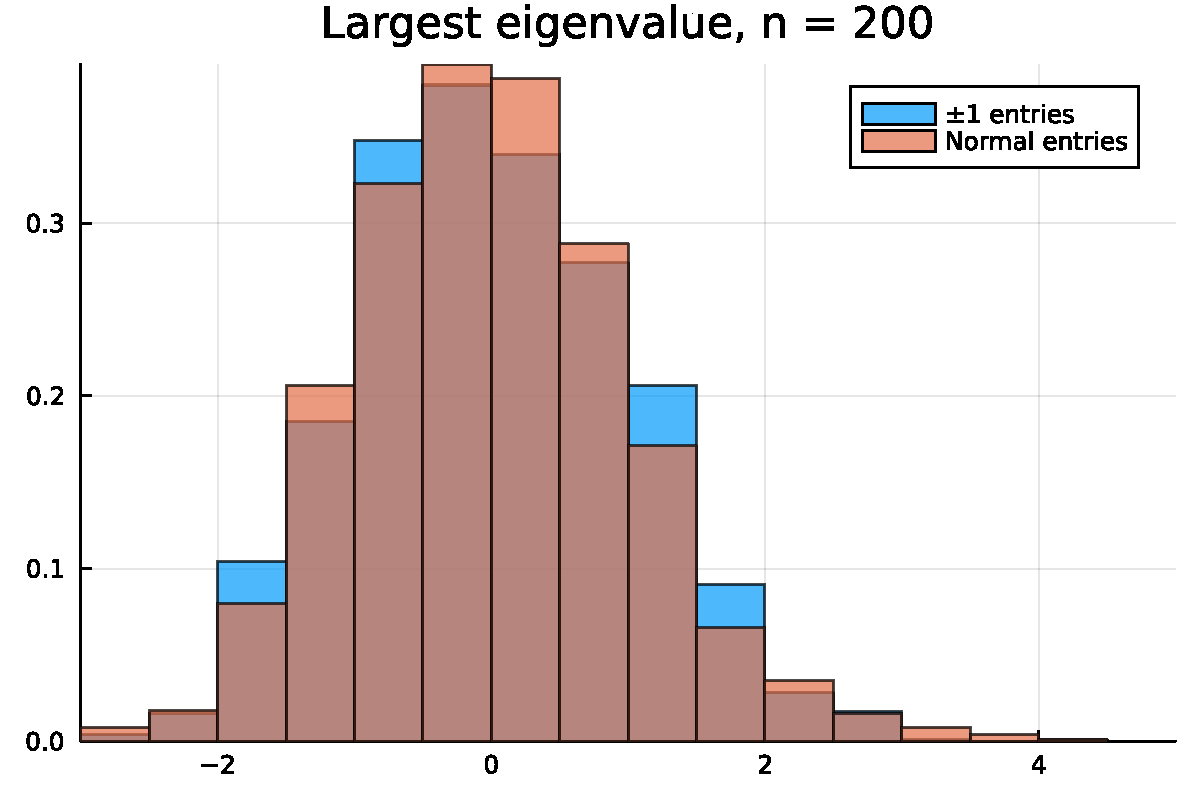
\includegraphics[width=0.6\linewidth,height=0.45\linewidth]{figures/II.Universality_3_1.pdf}

This distribution is known as the \href{https://en.wikipedia.org/wiki/Tracy\ensuremath{\endash}Widom_distribution}{Tracy\ensuremath{\endash}Widom distribution}. It has no simple formula but can be written either in terms of a Painlevé function (which solves a nonlinear ODE). 

\section{Poster projects}
The possibilities for projects related to universality are endless and I encourage you to think about an original idea. Here are some example projects to help guide you:

\begin{itemize}
\item[1. ] Give a detailed explanation of Catalan numbers and the full proof of the semicircle law.


\item[2. ] Other local statistics also exhibit universality, for example, the spacing between two eigenvalues in the \emph{bulk} (i.e. away from the edges of the semicircle). Explore this phenomena. 


\item[3. ] Hermitian random matrices also satisfy universality properties. How do histograms of their eigenvalue statistics (both global and local) compare to the symmetric case?


\item[4. ] A \emph{Wishart ensemble} is a random symmetric matrix $X X^\ensuremath{\top}$ where $X \ensuremath{\in} \ensuremath{\bbR}^{m \ensuremath{\times} n}$ is a rectangular matrix with random entries. It also exhibits universality but depending on the ratio $\ensuremath{\alpha} = m/n$, where the eigenvalue distributions tend to the \href{https://en.wikipedia.org/wiki/Marchenko\ensuremath{\endash}Pastur_distribution}{Marchenko\ensuremath{\endash}Pastur distribution}. Explore this phenomena and how $\ensuremath{\alpha}$ dictates which Marchenko\ensuremath{\endash}Pastur distribution arises. Does the largest eigenvalue still follow the Tracy\ensuremath{\endash}Widom distribution?


\item[5. ] The spacing of zeros of the Riemann Zeta function on the critical line match universality, in particular, the spacing of  eigenvalues in the bulk. Explore computation of zeros of Riemann Zeta functions (using eg. \texttt{scipy.special.zeta}) and compare with suitably-rescaled random matrix statistics.


\item[6. ] What happens when the moments are no longer defined? I.e. what are eigenvalue statistics for matrices with heavytailed entries?


\item[7. ] One can consider matrices associated with random networks, a la as discussed in Introduction to Applied Mathematics. If a network is completely connected it will be a Wigner ensemble. Explore experimentally how connected  a random network needs to be to exhibit universality.

\end{itemize}

